\chapter{Literature Overview}\label{chap:lit}
\begin{overview}
  A literature overview on model predictive control and controller constraints   is presented in this chapter.
Process operability is reviewed and the   operability index -- used as the basis for constraint interaction -- is   defined.  
Finally, a summary of the mathematical techniques used is given.
\end{overview}

\section{Model Predictive Control}\label{sec:mpclit}
Since its successful implementation in the petrochemical industry, model predictive control (MPC) has gained widespread acceptance in the processing sector \citep[1]{maciejowskimpc}. 
This has led to the development of many commercial MPC packages such as DMCplus (Aspentech), RMPCT (Honeywell), Connoisseur (Invensys) and SMOC (Shell Global Solutions) \citep{qinbadgwell}.
\subsection{Nomenclature and notation}
For the sake of coherence between sources a set nomenclature and notation scheme will be used. 
The following variables are defined; $x$ refer to the states of the system, $y$ to the outputs and $u$ to the inputs.
Where vectors are concerned (the MIMO case), a bold face character is used, e.g. $\vect{x}$ for $x$.
Matrices are distinguished by the use of capitals.

For discrete time forms, $k$ is used to denote the sample number.
For simplicity of notation, indices are used to refer to samples, i.e. $x_{k+1}$ instead of $x(k+1)$.
\subsection{Control theory}
Model predictive control differs from other model based control techniques (such  as Inverse Nyquist Array- and Internal Model Control) in its active use of predictions for future process outcomes \citep[137]{maciejowskifb}. 
In this context, MPC further distinguishes itself from other predictive control techniques in its ability to accommodate constraints on inputs and outputs.

\citet[8]{maciejowskimpc} summarises the control methodology of MPC in four steps; Measure, Predict, Optimize/Calculate and Apply. 
Along with figure~\ref{fig:mpc:general} these steps are summarized below;
%TODO - add symbols to list
\begin{enumerate}
  \item Measure; the current outputs are measured and the error (deviation from the set-point trajectory) is calculated.
  \item Predict; using the model, future outputs are calculated (over the prediction horizon).
  \item Optimize/Calculate; control moves (over the control horizon) are now calculated to minimize the predicted deviation from the set-point trajectory.
  \item Apply; only the first control move is implemented, where-after this procedure is restarted.
\end{enumerate}
\begin{figure}[htbp]
  \centering
  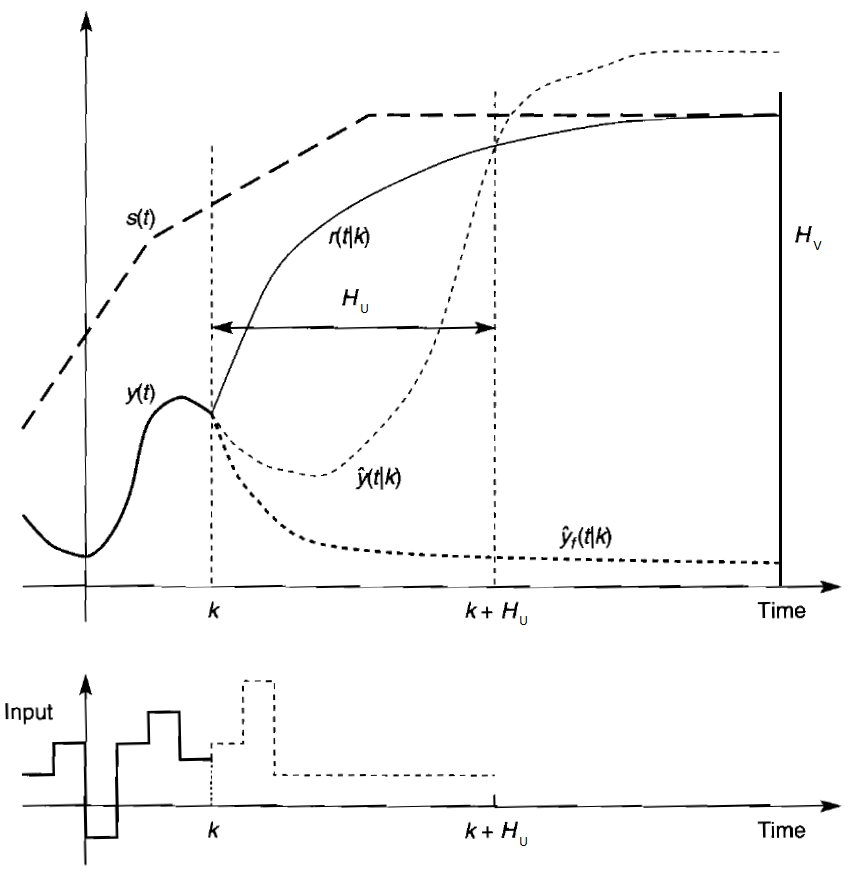
\includegraphics[width=8cm]{graph/mpc_general}
  \caption[General MPC working]{General MPC working, showing predictions on both outputs and inputs}
  \label{fig:mpc:general}
%TODO - fix figure to use coherent nomenclature
\end{figure}

\subsection{Models}
The correct choice of model is one of the most important steps in the operation of MPCs \citep[17]{rossiter}.
This is due to the active use of the model in making predictions as the controller runs, and not serving merely as an analysis aid \citep[37]{maciejowskimpc}.

\subsubsection{State space models}
State space models are the most encountered type in literature.
The general, linear, time-variant, state space model is presented in equation~\ref{eq:genss}.
\begin{align}
  \label{eq:genss}
  \ddfrac{\vect{x}}{t} &= A(t)\vect{x} + B(t)\vect{u} \notag \\
  \vect{y} &= C(t)\vect{x} + D(t)\vect{u} \\
  \vect{x}(0) &= \vect{x}_0 \notag
\end{align}
Where $A(t),~B(t),~C(t)$ and $D(t)$ are appropriately sized matrices of the state space model, and $\vect{x}_0$ is the initial state of the system.
For the time-invariant case, these matrices simply reduce to $A(t),~B(t),~C(t)$ and $D(t)$. 
As MPC is mostly implemented at discreet time steps, the model in equation~\ref{eq:genss} (for the time-invariant case) translates to equation~\ref{eq:genssdisc}.
\begin{align}
  \label{eq:genssdisc}
  \vect{x}_{k+1} &= A\vect{x}_k + B\vect{u}_k \notag \\
  \vect{y}_k &= C\vect{x}_k + D\vect{u}_k \\
  \vect{x}_0 &~ \text{(given)} \notag
\end{align}

\subsubsection{Step and pulse response models}
Step and pulse response models, especially finite impulse response (FIR) models, were widely used in the original descriptions of MPC.
There has, however, been a recent trend to move to other model types, such as transfer function models \citepp{113}{maciejowskimpc}{26}{rossiter}.

The pulse response model can be defined using the common convolution model \citep[284]{luyben}, as shown in equation~\ref{eq:fir}.
Where $H$ is a matrix representing the response of an output to a unit pulse in the corresponding input.
\begin{equation}
  \label{eq:fir}
  \vect{y}(t) = \sum^t_{k=0}H(t-k)\vect{u}_k
\end{equation} 
Even though the FIR models are intuitive they are not without shortcomings.
The most prominent of these problems are that FIR models are only applicable to asymptotically stable plants, and they are only adequate if the CVs are measured outputs.
\citet[109]{maciejowskimpc} elaborates on this topic.

\subsubsection{Transfer function models}
In the Laplace domain, the input/output relationship of a generic process (as shown in figure~\ref{fig:genmodel}) represented by
\begin{equation*}
  \vect{\bar y}(s)=G(s)\vect{\bar u}(s)
\end{equation*}
where $G$ is the process matrix, and $\vect{\bar u}$ and $\vect{\bar y}$ are the process inputs and outputs (in deviation variables) respectively.
The process matrix ($G$) can contain dynamic elements or, in the case of a steady-state model, only gains.
Note that state ($\vect{x}$) information do not appear in the transfer function formulation.
\begin{figure}[htbp]
  \centering
  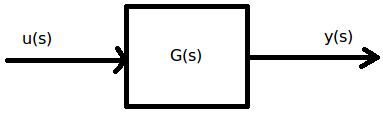
\includegraphics[width=8cm]{graph/model_genprocess}
  \caption[Generic input/output model]{Generic process showing inputs ($\vect{\bar y}$), model ($G$) and outputs ($\vect{\bar x}$).}
  \label{fig:genmodel}
\end{figure}
With the assumption of an initial zero state ($\vect{x}_0=0$), the state space description (the time-invariant case) can be converted to a transfer function description.
Taking the Laplace transform of equation~\ref{eq:genss}, and rearranging, results in equation~\ref{eq:gentf};
\begin{align}
  \label{eq:gentf}
    \vect{\bar x}(s) &= (sI-A)^{-1}B\vect{\bar u}(s) \\
    \vect{\bar y}(s) &= (C(sI-A)^{-1}B+D)\vect{\bar u}(s) \notag
\end{align} 
\subsubsection{Other model types}
Some other model types are used in MPCs, most are however derived from or reformulations of the above mentioned types.
Examples include; distributed models \citep[4]{rawlings}, CARIMA models and matrix fraction descriptions \citep[24,28]{rossiter} -- with the later two stemming from transfer function descriptions.

It should be noted that even though only linear models have been presented in this section, many MPCs are capable of using non-linear models.
The use of linear models in MPC is, however, common practice.
Important reasons for this are; no assurance of convergence of solutions and optimization being non-trivial for non-linear models \citep[17]{rossiter}.

\subsection{Objective functions}
Optimal control moves are determined by means of objective functions.
These functions are often referred to as cost functions \citep[41]{maciejowskimpc} as they can incorporate input/output weighting based on economic factors.

The general formulation of the unconstrained objective function is presented in equation~\ref{eq:genobjfn}. 
Modifications to this function (due to constraints) is discussed in section~\ref{sec:conobjfn}. 
From \citet[17]{rawlings} and \citet[41]{maciejowskimpc}, the objective function which penalizes deviations from the set-point trajectory as well as moves in the inputs is shown below;
% TODO - eqn in terms of zero setpoint, generalize to non-zero sp
\begin{equation}
  \label{eq:genobjfn}
  V(\vect{x}_0,\vect{u})=\frac{1}{2}\sum^{N-1}_{k=0}[\vect{x}_k'Q\vect{x}_k + \vect{u}_k'R\vect{u}_k]
  + \frac{1}{2}\vect{x}_N'P_f\vect{x}_N
\end{equation}
It is clear that the objective function depends on both the state sequence and the input sequence. 
The current state, $\vect{x}_0$ is known (measured) and the subsequent states are determined by the model and the input sequence. 
The optimal MPC control problem therefore becomes;
\begin{equation}
  \label{eq:opctrlprob}
  \min_{\vect{u}} V(\vect{x}_0,{\bf u})
\end{equation}

\subsection{Tuning}
As far as the objective function (equation~\ref{eq:genobjfn}) is concerned, the most prominent tuning parameters for MPC is the weighting matrices $Q$, $R$ and $P_f$. 
These are used to enforce the relative importance of deviations in both the inputs and outputs.

The weighting matrices are by no means the only tuning parameters for MPCs; additional parameters include the horizons used for predictions, the reference trajectory and the auxiliary models used (e.g. disturbance models). 
Chapter 7 of \citet{maciejowskimpc} covers the tuning of MPCs in some detail.

\section{Constraints in MPC}
The implementation of constraints is probably the most important selling point of MPCs.
When used in conjunction with a steady-state optimizer, MPCs are able to operate with more CVs than MVs \citet{vinsonphd}. 
Control of the CVs are now within ranges rather than on set-points.
% DO SOMETHING HERE

\subsection{Constraint types}
A multitude of constraints and constraint types are present in the MPC algorithm.
The following section lists these constraints and give a short description of their function and properties.
\subsubsection{Control constraints}
Often called ``hard'' constraints, these constraints are used for control (as opposed to optimization) and are never violated.
Control constraints exist for both outputs and inputs, and typically sort into two categories;
\begin{itemize}
  \item The constraints on inputs are typically physical constraints.
    Examples are valve saturation limits, tank levels and maximum heat      duties.
    Control constraints on outputs are usually concerned with safety and damage to equipment.
  \item Another class of control constraints (usually on outputs) are concerned with product quality and are thus operational in nature.
\end{itemize}

\subsubsection{Optimization constraints}
The constraints implemented by the optimizers in MPC are often called ``soft'' constraints.
These constraints are typically determined by operational and economical factors.
These constraints are usually implemented in two forms;
\begin{itemize}
\item Constraints to regulate dynamic behaviour, such as ``funnels''.
Examples of these are given in chapter~\ref{chap:background}.
\item Steady-state constraints which usually represent the optimal solutions of some external cost function.
The limits of these constraints are contained within the control constraints mentioned above.
\end{itemize}
As these constraints are usually not critical, situations exist where these constraints are violated in an attempt to ensure feasibility of the MPC solution.
This is discussed further in section~\ref{sec:coneffsol}.
 
\subsection{Constraint formulation}
Constraints on the inputs or outputs of a system can be represented as sets of linear inequalities.
For the most general case, they can be expressed as follows;
\begin{align}
  \label{eq:gencons}
  A_u\vect{u}_k &\leq b_u \notag \\
  A_y\vect{y}_k &\leq b_y \\
  A_x\vect{x}_k &\leq b_x \notag
\end{align}
where $A_u,~A_y$ and $A_x$ are coefficient matrices, and $b_u,~b_y$ and $b_x$ the half-space offsets.
For the case where only upper and lower bounds on variables exist, $A_u$ and $b_u$ reduce to;
\begin{align*}
  A_u={I\brack -I} \qquad b_u={\vect{u}^{max}_k \brack -\vect{u}^{min}_k}
\end{align*}
where $\vect{u}^{max}_k$ and $\vect{u}^{min}_k$ correspond to the upper and lower limits of $\vect{u}_k$ respectively \citep[6]{rawlings}. 
The coefficient matrices and offsets are reduced similarly for the outputs and the states.

For constraints on rate of change of inputs, the formulation is similar to equation~\ref{eq:gencons}.
The change in $\vect{u}_k$ during a sampling instance is now considered thus;
\begin{align*}
  A_{\Delta u}\Delta \vect{u}_k &\leq b_{\Delta u} \notag \\
  \text{and}~~ \Delta \vect{u}_k &= \vect{u}_{k+1}-\vect{u}_k
\end{align*}

\subsection{Constrained objective functions}\label{sec:conobjfn}
When constraints are present, the general objective function (equation~\ref{eq:genobjfn}), now subject to equation~\ref{eq:gencons} can be reformulated as a quadratic programming (QP) problem.
This makes the problem convex and has favourable consequences for the solution of the optimization (discussed in section~\ref{sec:coneffsol}).

The mathematical description of the QP problem is omitted from this dissertation, but \citet[81-83]{maciejowskimpc} as well as \citet[489-490]{rawlings} can be consulted for the complete reformulation.

\subsection{Effect on solutions}\label{sec:coneffsol}
As mentioned in section~\ref{sec:conobjfn}, the reformulation of the objective function and constraints into a QP problem -- and the subsequent convexity of the optimization -- affects the solution in numerous ways.
\citet[83]{maciejowskimpc} lists some of the solution properties obtained; namely that the termination of the QP problem is guaranteed and that computation time can be calculated.

Constrained optimization does however suffer from the problem of possible infeasibilities. 
For commercial MPCs the solvers are usually custom built to provide a ``back-up'' solution in the case of infeasibilities.
This back-up solution usually consists of modifying constraints (hence the term ``constraint handling'').
The most common methods of doing this are listed below;
\begin{itemize}
\item Constraint softening, where constraints are prioritized and then relaxed (or removed) until feasibility is obtained \citep[160]{rossiter}.
\item Using constraint windows which define a horizon over which constraints are enforced.
Feasibility can now be obtained by changing the start and end-time of this window \citep[281-282]{maciejowskimpc}.
\item Back offs and borders can be defined, effectively changing all constraints into ``soft'' constraints.
Due to the conservative approach, setting the back off amounts therefore becomes a feasibility assurance and performance compromise \citepp{161}{rossiter}{282}{maciejowskimpc}.
\end{itemize}

\section{Process Operability}
The method of constraint handling, as presented in this document, stems largely from work done by Georgakis and colleagues, in particular \citet{vinsonphd}, \citet{vinsonartoi}, \citet{limaphd}, \citet{opconproc} and \citet{opidealrx}. 
To place the operability index of \citet{vinsonphd} (defined in section~\ref{sec:oi}) in context, a short overview of the most common process operability techniques is presented below.

\subsection{Overview}
The subject of process operability is an ongoing field of study with many of the methods available being qualitative \citep[164]{skogestad}. 
A distinction is made between steady-state and dynamic operability methods. 
Whereas the later considers dynamic criteria, steady-state operability measures evaluate the relationship of process inputs and outputs at steady-state only.

\subsubsection{Steady-state operability measures}
The relative gain array (RGA) is one of the most used operability measures \citep[576]{luyben} and relates input/output interactivity.
Each element in the RGA ($\beta_{ij}$) is defined as the ratio of the steady-state gain ratios between input, $i$, and output, $j$, when all other inputs are constant and when all other outputs are constant.
\citet{artrdg} defined the RDG, which expanded on the RGA to include the effect of disturbances. 
Noting that the values of the RGA can be ``misleading'' \citep[87]{skogestad}, the use of norms such as the RGA-number are preferred.

The Niederlinski index is another measure that uses only steady-state gains of the process model \citep[572-573]{luyben}. 
This index is considered necessary but not sufficient, as positive values of the Niederlinski are inconclusive to the stability of the system \citep[445]{skogestad}.

Singular value decomposition stems from the use of eigenvalues as an operability measure. 
The use of singular values are preferred as eigenvalues are a poor
measure of gain and can often be misleading \citep[75]{skogestad}.
Maximum and minimum singular values are mostly used to select controlled variables but can also be used as a performance measure along with the condition number \citepp{596}{luyben}{80-82}{skogestad}.

\subsubsection{Dynamic operability measures}
The RGA can be expanded to contain frequency-dependant terms and is often referred to as the dynamic relative gain array (DRGA) \citep[637]{marlin}. 
The RDG \citep{artrdg} can be expanded in a similar way to include frequency-dependant terms.

Nyquist array methods as defined by Rosenbrock, as quoted by \citet[92]{skogestad}, are an extension of the SISO Nyquist stability criteria that include frequency dynamics. 
The two methods developed are the direct Nyquist array and the inverse Nyquist array. 
When used in conjunction with Gershgorin bands, conditions for overall stability can be derived \citep[440]{skogestad}.

\citet{vinsonphd} lists other dynamic operability measures which rely on the choice of a controller type. Further shortcomings of the above mentioned operability measures are also discussed in that text. 

\subsection{Operability Index}\label{sec:oi}
The operability index was defined by \citet{vinsonphd} as a measure of steady-state process operability. 
Constraint interdependence is used as the basis of this index. 
Further work by \citet{limaphd} expanded this index to cover non-square systems and some application to dynamic systems.
%% EXPAND
\subsubsection{Definitions}
The operability index focuses on input-output relationships rather the system's dynamic states \citep{vinsonphd}. 
Input and output values are defined by 'spaces' (in $\mathbb{R}^n$). 
These spaces are the 'feasible regions' which are bounded by the inequalities describing the ranges of the inputs or outputs. 
The following spaces are of interest;
\begin{itemize}
  \item Available Input Space (AIS); the set of values that process      inputs can take. 
    The limits on these values are based on both physical limits (e.g.     valve openings) or process design values (e.g. flow-rates or temperatures). 
Figure~\ref{fig:sampleais} illustrates an AIS for two variables ($u_1, u_2$) bounded by simple high/low limits.
  \item Achievable Output Space (AOS); this is the set of values which the process outputs can obtain, given the AIS. 
The AIS maps to the AOS by means of a process model, $G$. 
Therefore, a point $u$ in the AIS corresponds to a point $y$ in the AOS via $y=G(u)$. 
Examples of AOSs for linear and non-linear models are shown in figure~\ref{fig:sampleaos}.
  \item Desired Output Space (DOS); this represents the desired output values of the process. 
These values are typically based on operational and financial   parameters. 
Figure~\ref{fig:sampledos} shows a sample DOS for a two output    system.
  \item Expected Disturbance Space (EDS); all the values of the expected disturbances to the system. 
In the case of linear models, these values are translated back to the input space by means of a disturbance model, $G_d$.
  \item Desired Input Space (DIS); in the same manner that the AIS maps to the AOS, the DIS represents combined reverse mappings of the DOS and EDS.
The DIS is calculated as the inputs, $u$, that satisfy the model, ie. $y=G(u,d)$ (with $y$ and $d$ from the DOS and EDS respectively).
Figure~\ref{fig:sampledis} shows this combined translation.
\end{itemize}

%% MAYBE USE ONE BIG FIGURE FOR ALL SPACES?
\begin{figure}[htbp]
  \centering
  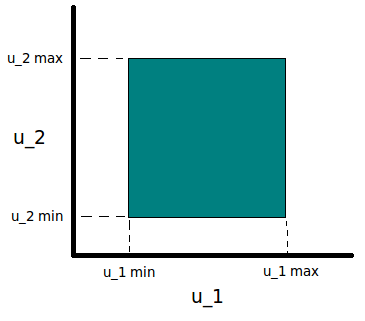
\includegraphics[width=8cm]{graph/sample_ais}
  \caption[Sample Available Input Space]{Sample Available Input Space (AIS) showing high/low limits on both inputs}
  \label{fig:sampleais}
\end{figure}

\begin{figure}[htbp]
  \centering
  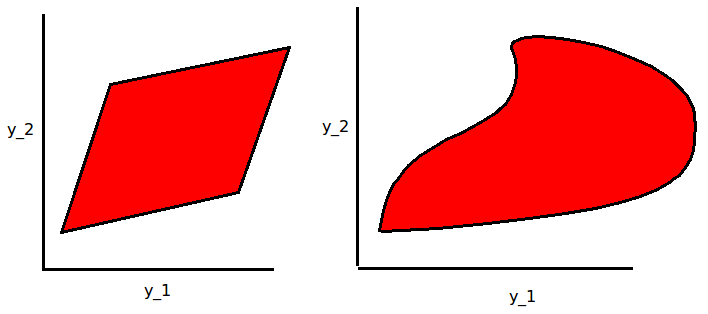
\includegraphics[width=8cm]{graph/sample_aos}
  \caption[Sample Achievable Output Space]{Sample Achievable Output Space (AOS)
    -- Linear model (left) and non-linear model (right)}
  \label{fig:sampleaos}
\end{figure}

\begin{figure}[htbp]
  \centering
  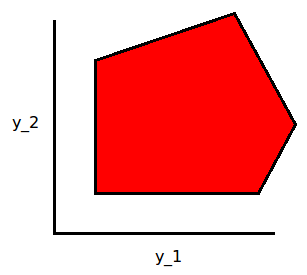
\includegraphics[width=8cm]{graph/sample_dos}
  \caption[Sample Desired Output Space]{Sample Desired Output Space (DOS) with 
    linear constraints on both outputs}
  \label{fig:sampledos}
\end{figure}

\begin{figure}[htbp]
  \centering
  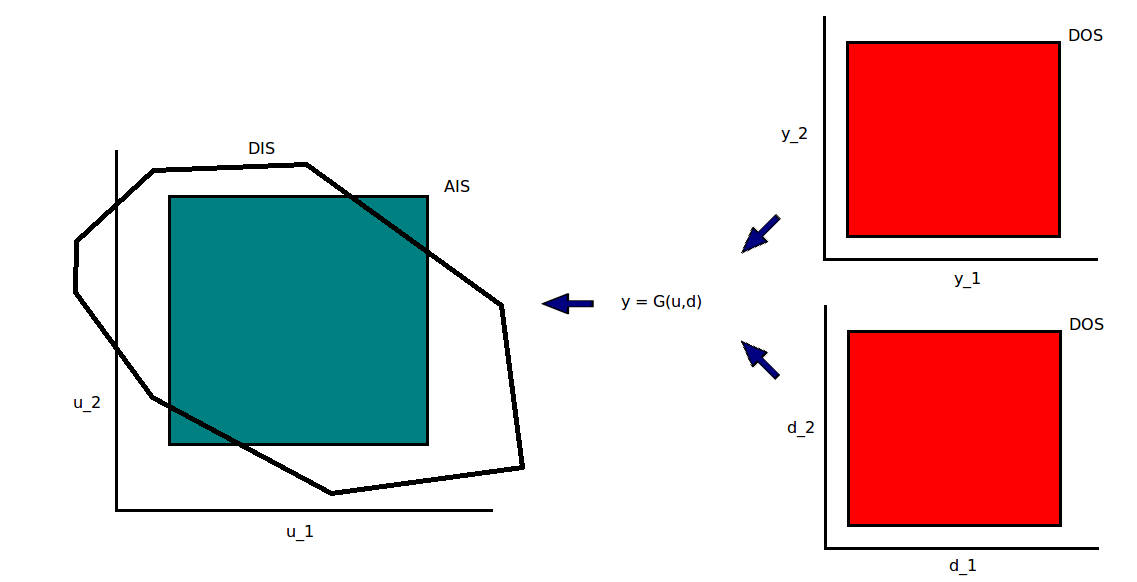
\includegraphics[width=8cm]{graph/sample_dis}
  \caption[Sample Desired Input Space]{Sample Desired Input Space (DIS) for
    a linear model and rectangular DOS and EDS}
  \label{fig:sampledis}
\end{figure}

\citet{vinsonphd} proceeds to define the generalised Output Operability Index (OOI) as shown in equation~\ref{eq:genooi}. 
Where $\mu$ represents a function to calculate the volume of a space.
From this definition it is clear that the controlability of a process decreases if the DIS does not cover the whole AIS. 
Servo- and regulatory operability indices are also defined in the text, but are not shown here.
\begin{equation}
  \label{eq:genooi}
     OOI = \frac{\mu(AIS\cap DIS)}{\mu(DIS)}
\end{equation}

All the concepts above are directly applicable to square systems.
For the case of non-square systems (more outputs than inputs) the operability index formulation is extended to interval operability. 
In this case, process outputs are split into two categories; setpoint controlled variables and range controlled variables.
The first being controlled on a given setpoint, whereas the later is allowed to vary within its given maximum and minimum limits.

\citet{limaphd} elaborates on the interval operability of linear non-square systems and defines the following concepts:
\begin{itemize}
  \item The interval AOS (AOS$_I$); which is the union of all AOS($d$) where is within the EDS. 
This is typically generated by the shifting of AOS($d=0$) in the directions determined by $G_d$ (the disturbance model).
  \item The Achievable Output Interval Set (AOIS); defined as a rectangle with the same aspect ratio as the DOS, bound by the lines (or hyperplanes) that correspond to the minimum and maximum values of $d$ in the AOS. 
Noting that the issue of interval operability is being addressed, the AOIS does not need to be strictly contained within the AOS$_I$.
\end{itemize}
The thesis of \citet{limaphd} proceeds to define a hyper-volume ratio (HVR) as shown in equation~\ref{eq:hvr}. 
The aim being here to define a measure for obtaining tighter control on CVs by reducing the size of the DOS (without causing infeasibilities). 
The process remains interval controllable as long as the AOIS remains a subset of the DOS (AOIS$\subseteq$DOS).
\begin{equation}
  \label{eq:hvr}
    HVR = \frac{\mu(DOS)}{\mu(AOIS)}
\end{equation}
To change the relative importance (tightness of control) on variables, weights are imposed on the AOIS. 
This in turn affects the aspect ratio of the AOIS.

\citet{limaphd} proposes two methods to calculate an AOIS for higher dimensional systems; an iterative method and a method based on linear programming. 
In both cases, this corresponds to the tightest set of output constraints which still render the system controllable. 
Both methods are briefly discussed below;
\begin{itemize}
  \item Iterative approach; this method relies on the use of computational geometry tools to calculate convex hulls and intersections. 
An AOIS is initially estimated and expanded until it intersects the extreme subsets of the AOS. 
The magnitude by which the AOIS is increased is calculated using the Secant and bisection method. 
The calculations contained in this method are computationally intensive and limit its use to systems of 8 dimensions and lower.
  \item LP approach; in this approach the constraints and objective function are reformulated as linear functions. 
The extreme subsets of the AOS are expressed as linear inequalities and objective function set up as to determine the common intersection point of the AOIS and a given extreme subset. 
The proposed LP approach overcomes the computational intensity of the iterative method and is suitable for on-line calculation of the AOIS.
\end{itemize}

\subsubsection{Application}
Numerous authors have illustrated the application of the operability index (OI). 
\citet{opconproc} focus on a general application of the OI, emphasising its ability to identify inoperable processes without the need to specify a controller structure. 
\citet{opidealrx} applies the OI to the design of ideal reactors. 
The analysis of a vinyl acetate reactor produced interesting results
regarding the mapping of the AIS to the AOS. 
It was shown that for certain classes of non-linear systems, the AIS boundaries do not map to the boundaries of the AOS.

Although the  operability index can be used with square or non-square, linear or non-linear models, its easiest application is to linear models. 
This is advantageous as most of the current MPCs use linear models \citep{vinsonphd}.

\citet{vinsonphd} highlights some properties of MPC (in particular DMCplus) which lends themselves to the  application of the operability index.
Table~\ref{tab:mpcoi} summarises these properties and applications.
\begin{table}[htbp]
  \centering
  \caption[Application of the operability index to MPC]{Application of the
    operability index to MPC \citep{vinsonphd}}
  \label{tab:mpcoi}
    \begin{tabular}{p{6cm} p{9cm}}
      \toprule
      MPC property & Operability index property \\
      \midrule
      Linear process models & Calculation of the relevant spaces (AOS and DIS) is usually fast.\\[1.3ex]
      Constraints on MVs and CVs & In the case of fixed constraints; the input/output constraints result in polytopes in both the input/output spaces. 
From these descriptions the framework of operability index can be directly applied.\\[1.3ex]
      Solution of MV and CV steady state targets  & Where an LP solver is used, the operability index can yield useful information about process characteristics.\\
      \bottomrule
    \end{tabular}
\end{table}

\section{Mathematical Preliminaries}
Some mathematical concepts are briefly covered in this section.
Their application is discussed in chapter~\ref{chap:prog}.
\subsection{Convex geometry}
Noting that only convex sets are considered in this project, many properties of convex geometry can be exploited.

The following nomenclature is reviewed and used throughout this document \citep[487]{bayerlee};
\begin{itemize}
\item polytope - the intersection of closed half-spaces in $\mathbb{R}^n$.
A polytope of $n$ dimensions will simply be referred to as an $n$-polytope.
\item vertex - a 0 dimensional face of an \npoly.
\item facet - an $n-1$ dimensional face of an \npoly.
\end{itemize}

\subsubsection{Half-space geometry}\label{sec:hgeometry}
Linear constraints (as described in equation~\ref{eq:gencons}) are equivalent to half-spaces in $\mathbb{R}^n$ in both their mathematical description and meaning.
From this we can conclude that all polytopes generated by linear constraints (half-spaces) are convex, as they have supporting hyperplanes at each boundary point \citep[21]{manilev}.
From this it also follows that the intersection of such convex polytopes will be convex.
This is due to the resulting intersection being merely a subset of the half-spaces defining the two intersecting polytopes.

The problem of degeneracy can occur when constructing polytopes from half-spaces.
Degeneracy is defined when objects ``change their nature to belong to another, usually simpler, class'' \citep[688]{crcmaths}.
For the purposes of this dissertation, the degeneracy of polytopes is important.
When the number of half-spaces used to construct a polytope is more than the final number of facets on the resulting closed polytope, the polytope is classified as degenerate.

\subsubsection{Convex hull and vertex enumeration}
The convex hull or facet enumeration is used extensively for calculations in this project.
It is defined as the smallest convex set containing $P$ if $P$ is a set of points ($P \subseteq \mathbb{R}^n$) \citep[74]{wenger}.
In this project, $P$ is generated from a set of half-spaces and the resulting vertices are the minimum vertex description of $P$.
For this reason the convex hull of $P$ and the half-spaces used to generate $P$ are equivalent.

The opposite of facet enumeration is vertex enumeration, where a set of half-spaces is transformed to the vertices of $P$.
A primal-dual method can be implemented to solve this problem.
A simplified description of the primary steps of this algorithm is given below (for $P$ defined by $A\vect{x}\leq\vect{b}$);
\begin{itemize}
\item Solve for an internal point in $P$.
\item Generate vectors normal to the half-spaces defining $P$, centered around the origin.
\item The convex hull of the vertices associated with these vectors are calculated.
\item The facet enumeration of this hull is then used to calculate intersections of half-spaces in the original $A$ matrix.
\item Duplicates are then removed and the vertices shifted back around the calculated inner point of $P$.
\end{itemize}
The full mathematical formulation of the primal-dual algorithm is omitted from this document.
\citet[636-639]{primaldual1} and \citet{primaldual2} can be consulted for the full formulation. 

\subsubsection{Linear transformations}
Defining $X$ and $Y$ as finite-dimensional sets with bases $(x_1,\cdots,x_n)$ and $(y_1,\cdots,y_m)$ respectively.
For the linear transformation $\phi : X \to Y$, the following holds;
\begin{equation}
  \label{eq:lintrans}
  \phi(x_i) = \alpha_{i1}y_i+\cdots+\alpha_{in}y_n \text{~~~for~} i = 1, \cdots, m
\end{equation}
The scalars $(\alpha_{ij})_{i=1,\cdots,n;~j=1,\cdots,m}$ can be written as
\begin{equation}
  \bpm
    \alpha_{11} &\cdots &\cdots &\alpha_{1n} \\
    \alpha_{21} &\cdots &\cdots &\alpha_{2n} \\
    \cdots     &\cdots &\cdots &\cdots \\
    \alpha_{m1} &\cdots &\cdots &\alpha_{mn} \\
  \epm \notag
\end{equation}
which is referred to as the matrix of $\phi$ \citep[48-49,~166]{leung}.

Equation~\ref{eq:lintrans} is equivalent to the result of the following matrix multiplication
\begin{equation}
  \label{eq:matmult}
  \Phi X = Y
\end{equation}
where $\Phi$ is the matrix of $\phi$.
Equation~\ref{eq:matmult} confirms that matrix multiplication is indeed a linear transformation.

\subsection{Process models}
The mathematical description of the process models considered in this project are shown below.
\subsubsection{Linear steady-state}
The steady-state model of a linear system is the gain-matrix.
This is simply a matrix of constants in $\mathbb{R}$.
Models like these allow for matrix algebra when transforming between the input and output spaces (and vice versa).
Obtaining the AOS from the AIS (as shown in figures~\ref{fig:sampleais} and~\ref{fig:sampleaos}) is a simple matrix multiplication of the vertices of the AIS and the process model matrix.
\subsubsection{Non-linear models}
An advantage of using linear models is that the surface (or boundary) of the input space (a polytope) maps directly to the surface of the output space.
For this reason, the constraints specifying the input space can be used to generate the output space with full mathematical rigour.

This is, however, not the case for non-linear models.
\citet{opidealrx} illustrates this for a vinyl acetate reactor where a set of inputs map to the same point in the output.
This phenomena of input multiplicities can be ascribed to rank deficiency of the Jacobian matrix of the process model.   

% Local Variables:
% TeX-master: "AHC_thesis"
% End: